\section{System design}
\label{sec:system_design}
~

No supervised learning model has been found in the literature to 
tackle the non-preemptive, global fixed-priority scheduling problem of a single DAG task.
That is because supervised learning is most often used for problems
that we, humans, know how to solve, but don't have an algorithm for it
and don't want to waste time solving it ourselves,
such as image classification or text classification.
In this case, there are ways to compute solutions to the problem
using linear programming, but it is costly and doesn't scale well 
when increasing the number of nodes per DAG.
Hence, in the literature, only reinforcement learning has been
used to tackle this problem, a machine learning method that 
doesn't need to know the true solution but 
can instead approximate the solution by maximizing a reward function.
Still, supervised learning is a widely used machine learning method
and can provide good interpretations when the model is not too deep.
Also, once trained, the supervised machine learning model can be 
fast and scalable in terms of computing time, unlike the ILP method.
Therefore, the supervised learning model's purpose will be to
approximate the computation of a priority-list for a single DAG task, 
that leads to the minimum makespan.

\subsection{Supervised design}
~

In supervised learning, 
the model predicts a value (forward pass) that is then compared to the known-to-be-true value using a
specific error-function, often called the loss function,
and the error is then propagated through the model to tweak its parameters, minimizing the loss function
(Figure \ref{fig:supervised_learning}).
The idea is, then, to treat the problem as a classification problem,
where each node of a DAG needs to be 'classified' in a specific priority.
ILP will be used to compute the optimal\footnote{Here and in the following paragraphs, 'optimal' means 'yielding the minimum makespan'.}
priority-lists, and use them as the known-to-be-true values to compare the model-predicted values with.


\begin{figure}
    \centering
    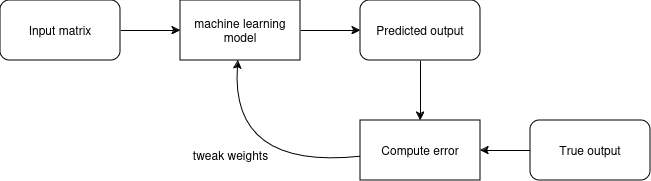
\includegraphics[width=\linewidth]{images/supervised_learning_diagram.drawio.png}
    \caption{The supervised learning method.}
    \label{fig:supervised_learning}
\end{figure}



\subsubsection{Input DAGs}
~

In machine learning, the input that we give to the model
needs to be in a matrix representation so that the model can 
then process it. Therefore, every DAG task needs to have
a matrix representation that encompasses information 
about its internal structure as well as its global attributes.  
Each input DAG task will, thus, be represented using 
a matrix of numbers with each row being a node
and each column being a raw feature of a node.
The list of raw features is similar to what is proposed by \citet{Lee2021GlobalDagSchedDRL},
that is :
\begin{list}{}{}
    \item - the normalized wcet of the node, i.e., $C_i / vol(G)$ for node $i$ ;
    \item - the number of incoming neighbours, i.e., predecessors ;
    \item - the number of outgoing neighbours, i.e., successors ;
    \item - a boolean value of whether the node is the source or sink node ;
    \item - a boolean value of whether the node is part of the critical path of the DAG.
\end{list}

The wcet is widely used as a criteria for priority-list scheduling algorithm (RM, EDF\cite{buttazzo2005RMvsEDF}, etc.)
but it needs to be normalized to have the context information of the whole graph.
The number of incoming and outgoing neighbours makes it possible 
to take into account the inner structure of the graph to compute the execution order.
The source and sink nodes are particular nodes in that their priority
is not important because they will respectively execute first and last due to their dependency constraints.
Finally, the critical path plays a huge role in state-of-the-Art heuristics\cite{He2019DagIntra}\cite{zhao2020DAGsched},
with nodes in the critical path often having higher priorities than those
that aren't.
An example of such a DAG task representation is shown in Figure \ref{fig:dag_task_matrix_example}.

\begin{figure}
    \centering
    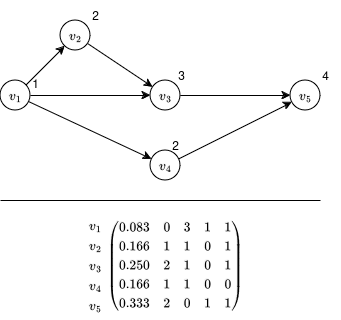
\includegraphics[width=\linewidth]{images/dag_matrix_example.drawio.png}
    \caption{Example DAG task with 5 nodes, a total workload of 12
    and the matrix representation of each node with the columns respectively representing the above list of features.}
    \label{fig:dag_task_matrix_example}
\end{figure}

\subsubsection{Output priorities}
~
\label{sec:output_labels}

In order for the supervised model to learn, it needs to 
compare its predicted output against a known-to-be-true output, also 
called an output label. In this case,
the problem is treated as a classification problem which means 
that for each node of a DAG, the model needs to output the probability
of this node being classified as a specific priority.
Therefore, for a DAG task with $n$ nodes,
each node must have a list of $n$ probabilities,
with each one being the probability of the node being 
assigned the priority corresponding to the position of the probability in the list
of probabilities, starting from 0.
For instance, if $n = 3$, 
a possible output for a node $v_i$ would be
$\text{model}(v_i) = [0.2,0.5,0.3]$ which means that according to the model,
the node $v_i$ has a probability to be assigned priority 0 of $0.2$,
priority 1 of $0.5$ and priority 2 of $0.3$.
As a consequence, the priority chosen for node $v_i$ will be 
the one that has the maximum probability a-posteriori (MAP strategy),
in the example above, it is priority 1.

This must be the case for every node and as the input 
is a matrix representing the whole graph, 
the output then also needs to be a matrix with 
each row corresponding to each node and the columns
correspond to the priorities, e.g., Figure \ref{fig:dag_output_matrix_example}.
\\

The model output needs to be compared to the known-to-be-true output or label,
which means we need a way of calculating the optimal priority list.
The idea is to use an ILP solver to compute the optimal schedule 
of a DAG task, and then use this optimal schedule to retrieve 
the optimal priorities for each node, according to their start time
in the computed schedule.
Each node will be sorted according to their start time, in increasing order,
and the priority value will then be the position of each node in the sorted list.
As a consequence, the node with the lowest start time will
have the highest priority.

The makespan calculation is done using a non-preemptive GFPS,
with a first fit core assigning strategy (see Section \ref{sec:makespan_calculation}). Hence,
the retrieved optimal priority list can sometimes 
lead to a different schedule than what the ILP solver computed.
Fortunately, because we're on a homogeneous system,
as long as the priorities are respected, the core assignment 
doesn't matter and would just lead to having a symmetric schedule
compared to the ILP schedule,
that is swapping cores in the ILP schedule, which doesn't change the makespan.

Therefore, an Integer Linear Programming (ILP) solver will be used to compute
the optimal schedule for each DAG task (see Section \ref{sec:ilp_calculation}) and then
ordering the nodes according to their start time in the ILP schedule,
thus having an optimal list of priorities for the nodes that can then be compared to
the predicted model output list.

\begin{figure}
    \centering
    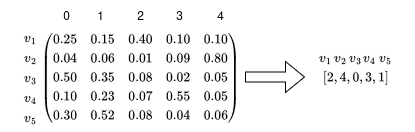
\includegraphics[width=\linewidth]{images/output_matrix_example.drawio.png}
    \caption{Example of an matrix output from the model, the predicted list of priorities (on the right)
    is retrieved from the probabilities using the maximum-a-posteriori (MAP) strategy.}
    \label{fig:dag_output_matrix_example}
\end{figure}

\subsubsection{Loss function}
~
\label{sec:loss_design}

Although the problem is being treated as a classification problem,
the goal still is to compute a priority list that minimizes the makespan
of the DAG.
Therefore, the idea was, initially, to compare the makespan
produced by the predicted priority-list with the makespan
produced by the ILP schedule, using a simple difference operator.
This difference would have been the loss function of the model : 
$loss(p_{\text{model}}, p_{\text{ilp}}) = |GFPS(p_{\text{model}}) - GFPS(p_{\text{ilp}})|$
with $p_{\text{model}}$ and $p_{\text{ilp}}$ being 
the priority lists outputed by the model and the ILP solver respectively.
Unfortunately, the non-preemptive GFPS which is used to compute the makespan,
isn't differentiable for the priority-list given to it,
which lead to segfaults in the training phase.
The segfaults happen because the non-differentiability 
of this loss function makes the PyTorch gradient calculation algorithm
try to compute something that doesn't exist.
Thus, instead of looking at the makespans,
the idea is to look at the priority matrix 
and compare the one predicted by the model to
the ILP priority matrix that is retrieved from the priority-list.
Indeed, an ILP output matrix to compare the predicted output to
can be calculated using the previously retrieved priority-list.
Like the model-predicted output matrix,
the ILP matrix output will represent the probabilities
of each node being assigned a specific priority, using the 
same process described in the previous section but in reverse, with a probability of 1 
on the optimal priority value, and 0 otherwise. 
For instance, if the optimal priority list for a DAG task of 3 nodes 
is [$v_1$: 0, $v_2$: 2, $v_3$: 1],
then the true label is the matrix :
$$
\begin{pmatrix}
    1 & 0 & 0\\
    0 & 0 & 1\\
    0 & 1 & 0
\end{pmatrix}
$$
With each row representing $v_1$, $v_2$ and $v_3$ respectively,
and the column representing the priorities 0, 1 and 2 respectively.

Once we have the two matrices, 
it is then possible to use the binary cross-entropy loss function,
widely used for classification problems,
to compare the predicted output to the optimal ILP matrix.

More specifically, the binary cross-entropy loss function is defined as :
\begin{equation}
    loss(x, y) = \sum_{i=1}^{n} -y_i\log(x_i)
\end{equation}
    
where $x$ is the flattened matrix representing the predicted output,
$y$ is the flattened matrix representing the true output (ILP output),
and $n$ is the number of elements in $x$ and $y$.


\subsection{Model design}
~
\label{sec:model_design}

The main idea for designing the architecture of the model is 
to leverage the structural information of the DAG.
That is, it needs to learn the relationships and connections
between the nodes to correctly classify the nodes into the right priorities.
In machine learning a prevalent architecture when dealing with graphs
is the graph neural network architecture.
The idea is, instead of treating each node as independent vectors, like 
in a traditional feed-forward network, 
a graph neural network gathers information of each node and its neighbours 
and passes it to the next layer.
One way to do that is to aggregate the neighbours' information of a node
and use this aggregation to compute the next representation vector of the node.

Unfortunately, this kind of aggregation also means that a node will have a 
vector representation similar to its neighbours, when passing through multiple layers of a graph neural network (GNN).
This problem can lead to groups of neighbours having very similar vector representations
and can cause an over-smoothing problem\cite{chen2020oversmoothing}.
The two main ways to fix this kind of problem is either to reduce the amount of GNN layers 
or/and use the attention-mechanism to give a notion of importance to a node's neighours,
thus reducing the impact a less important neighbour can have on the aggregation phase.
Of course, reducing the number of GNN layers also means less complexity which can decrease the performance of the model,
thus, a balance between having complexity and limiting the over-smoothing problem is often done to maximize performance.
This is exactly what they do in the literature\cite{Lee2021GlobalDagSchedDRL}\cite{Zhao2024GATDRLmodel}.
More specifically, \citet{Lee2021GlobalDagSchedDRL} designed a Graph Convolutional Network (GCN) based on the attention-mechanism
to encode the nodes' feature vectors in their reinforcement learning model, performing slightly better than the state-of-the-Art
heuristics from \citet{zhao2020DAGsched}.

Therefore, the model's architecture will be based on the proposed encoder in \citet{Lee2021GlobalDagSchedDRL},
and it will be comprised of three modules :
two feed forward networks and one attention-based graph convolutional network (GCN) (see Figure \ref{fig:model_diagram}).

\begin{figure}
    \centering
    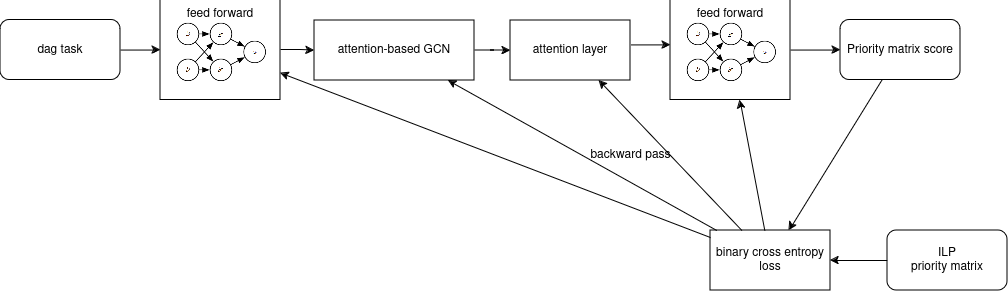
\includegraphics[width=\linewidth]{images/designed_model.png}
    \caption{The architecture diagram of the proposed supervised machine learning model.}
    \label{fig:model_diagram}
\end{figure}

\subsubsection{Feed forward networks}
~

Using a feed-forward network (FFN) before the GCN can help at pre-encoding the feature vectors of the nodes
so that the GCN can better work on those feature vectors.
Also, a feed-forward network (FFN) at the end of the model is needed to make 
the final classification decision about each node, once the feature vectors have
all the graph structural information encoded into them.
Of course, the more layers in the FFN, the more complexity
is encoded in the feature vectors, but it can also potentially lead to an over-fitting
problem with the model being too complex and taking noise information into account,
decreasing its generalization power and its overall performance.

Therefore, the two feed forward networks will have 3 layers with each 
layer $n$ producing the following output,
\begin{equation}
    o_{n} = ReLU(W_{n}X_{n} + b_n),\, n \in \{1,2,3\}
\end{equation}
where $W_n \in \mathbb{R}^{5\times5}$ is the matrix of trainable weights
at layer $n$, $b_n \in \mathbb{R}^5$ is the bias, $X_n$ is either a node's vector representation
or the output of the previous layer, and $ReLU(x) = max(0, x)$.
There is an exception for the second feed forward network where the last 
layer's output is computed using the following equation:
\begin{equation}
    o_{3} = \sigma(W_{3}X_{3} + b_3)
\end{equation}
where $W_3 \in \mathbb{R}^{nbPriorities \times 5}$,
$b_3 \in \mathbb{R}^{nbPriorities}$ and $\sigma$ is the 
sigmoïd activation function.
Also, $nbPriorities$ corresponds to the number of different priorities
that can be assigned to each node, which in this case is going to be the same as the number of nodes in the input DAG.


\subsubsection{Graph Convolutional Network}
~

The GCN layer needs to aggregate the information 
of the neighbours of a node and use that information
to compute the next representation vector of the node.
To do that, we utilize both the incoming and outgoing neighbours
of a node and compute their attention scores to then aggregate
that information and pass it through an activation 
function, thus updating the representation vector of the node (see Figure \ref{fig:update_aggregate_diagram})
Considering both in and out neighbours enables the structural complexity 
of the graph to be better encoded, and also
uses the directed aspect of the DAGs.
The Figure \ref{fig:update_aggregate_diagram} represents
one GCN layer.

To be more specific, for each GCN layer, the input vector $X^{v_i}_k$ 
goes through an aggregation phase where,
the inputs are the set of incoming neighbours of node $v_i$, $\mathcal{N}_{in}(v_i)$, which includes
$v_i$, and the set of outgoing neighbours $\mathcal{N}_{out}(v_i)$, which also includes $v_i$,
and the output is
the next vector representation $X^{v_i}_{k+1}$, calculated by the following equation:

\begin{equation}
GCN(X) = AttentionModule(X, \mathcal{N}_{in}(v_i), \mathcal{N}_{out}(v_i))
\end{equation}

where $AttentionModule$ is defined by the Equations \ref{eq:attention_module}--\ref{eq:elu}
and computes the importance scores of each neighbour, in each set of neighbours.
$X^{v_i}$ is the feature vector for the node $v_i$.

\begin{multline}
    AttentionModule(X, \mathcal{N}_{in}(v_i), \mathcal{N}_{out}(v_i)) = \\
    ELU\left( W \left( Att(X, \mathcal{N}_{in}(v_i)) \oplus Att(X, \mathcal{N}_{out}(v_i)) \right) + b \right)
    \label{eq:attention_module}
\end{multline}

\begin{equation}
Att(X, \mathcal{N}(v_i)) = W\sum_{j \in \mathcal{N}(v_i)} \alpha_{ij} X^{v_j}
\label{eq:attention_submodule}
\end{equation}
Where 
\begin{equation}
    \alpha_{ij} = \frac{\exp \left ({ a ^{T} W X^{v_i} + b ^{T} W X^{v_j} }\right )}
    {{\sum _{k \in \mathcal {N}(v_{i})}} \exp \left ({ a ^{T} W X^{v_i} + b ^{T} W X^{v_k} }\right )}
\end{equation}

are the attention coefficients
which evaluates how important is $v_j$ to $v_i$'s vector 
representation, similar to what is done in \citet{Lee2021GlobalDagSchedDRL}.
Equation \ref{eq:attention_submodule} computes the attention scores
for each neighbour of node $v_i$, 
scores that are then used in Equation \ref{eq:attention_module}
to aggregate the scores information and pass it through 
the ELU activation function.
Every $W$, $a$, and $b$ are different matrices of trainable parameters,
and $\text{ELU}$ is the exponential linear unit activation function (Equation \ref{eq:elu}).

\begin{figure}
    \centering
    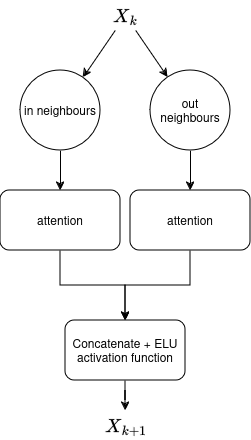
\includegraphics[width=0.5\linewidth]{images/gcn_update_aggregate_diagram.png}
    \caption{Diagram of the graph convolution network layer. $X^{v_i}_k$ is the transformed node vector representation,
    for node $v_i$,
    and ELU is the exponential linear unit function (see Equation \ref{eq:elu}).}
    \label{fig:update_aggregate_diagram}
\end{figure}

\begin{equation}
\text{ELU}(x) = 
\begin{cases}
x, & \text{if } x > 0 \\
\exp(x) - 1, & \text{if } x \leq 0
\end{cases}
\label{eq:elu}
\end{equation}


The GCN layer can be repeated several times 
to improve the model's capacity to
capture the complexity of the graph structure.
In this case, the number of GCN layers was set to 3.

\subsection{Computing the labels}
~
\label{sec:ilp_calculation}

\subsubsection{Computing the optimal schedule}

ILP will be used to compute the optimal schedule,
hence the need to have an ILP solver.
Fortunately, 
\citet{yip2023letsynchronise} proposed an ILP-based
scheduling solver for event-chains of time-triggered tasks
using the Logical Execution Time paradigm\cite{kirsch2012logical}.
Their work aimed at minimizing the sum of dependency delays 
between the job instances of each task and they have recently added
support for multicore architectures\footnote{https://github.com/mkuo005/LET-LP-Scheduler}.

Although their minimizing problem is slightly different from ours, 
we can convert our minimizing problem and then use their LET solver by converting each DAG task 
to an event-chain of LET task.
To do this, each node needs to be converted to an LET task which 
implies adding an initial offset, activation offset, LET interval duration and a period
to every node.
Hence, for each node, the initial offset and activation offset will
be set to 0 and the LET interval duration will be set to the node's wcet.
For the period, every node in a DAG will have the same period which will
be equal to the total workload squared.
The wcet of a node will be the wcet of its LET task version.
Lastly, each path in the DAG will represent an even-chain of tasks.

Unfortunately, minimizing the sum of dependency delays (i.e., Equation 6 in \citet{yip2023letsynchronise}) is not equivalent
to minimizing the makespan of a DAG (see Figure \ref{fig:counter_example_minsumdep})
but we can change the objective function to the end execution time
of the sink node, i.e., the node which doesn't have any successors,
which is the definition of the makespan.
This effectively makes the solver minimize the makespan of DAG task
which is precisely the problem at stakes\footnote{See the github repository for more details \url{https://github.com/FelicienFG/research-project-AUT/}.}.

\begin{figure}
    \centering
    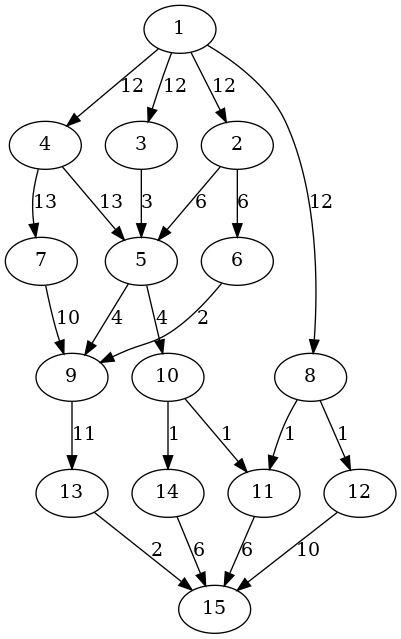
\includegraphics[width=0.5\linewidth]{images/Tau_108.png}
    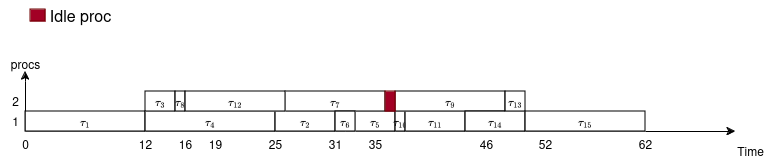
\includegraphics[width=\linewidth, height=70px]{images/schedule_example_ilpfail_correct.png}
    \par Schedule a)
    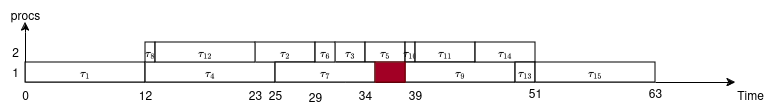
\includegraphics[width=\linewidth, height=55px]{images/schedule_example_ilpfail_better.png}
    \par Schedule b)
    \caption{Example of a DAG task (top image) where the schedule that the ILP solver outputs (the schedule a))
    produces a longer makespan (64) but smaller sum of dependency delays (400) than 
    the schedule b) with a makespan of 63 and a sum of dependency delays of 427.}
    \label{fig:counter_example_minsumdep}
\end{figure}

\subsubsection{Computing the optimal priority-list}
~

Once the optimal schedule (i.e., the schedule yielding the minimum makespan)
is computed,
the optimal priority-list can be obtained from the schedule 
by looking at the start times of each node and incrementing the priority value
according to the node's start time.
The sooner the start time, the higher the priority.

For instance, for the non-optimal schedule shown in Figure \ref{fig:counter_example_minsumdep} (schedule a)),
the corresponding priority-list would be 0 for node $v_1$, 1 for node $v_4$,
etc, i.e., [$v_1$: 0, $v_2$: 3, $v_3$: 2, $v_4$: 1, $v_5$: 4, $v_6$: 6, $v_7$: 5, $v_8$: 8,
 $v_9$: 10, $v_10$: 7, $v_11$: 9, $v_12$: 11, $v_13$: 13, $v_14$: 12, $v_15$: 14].
This priority list is then converted to a matrix by the process described
at the end of Section \ref{sec:output_labels}.

\subsection{Makespan calculation}
~
\label{sec:makespan_calculation}

The main performance metric that will be used in the evaluation
is the makespan, i.e., the end execution time of the sink node of a DAG.
The exact computation of the makespan is done by simulating a 
simple non-preemptive global fixed-priority scheduler, for which the algorithm
is described in the Figure \ref{fig:algo_makespan}.
The basic idea is to have a ready queue that contains the nodes
that have their precedence constraints met
and the nodes still waiting to have their dependencies met 
are in the waiting list. At each loop iteration, the waiting list and ready queue
are updated and the first idle processor gets the node at the top of 
the ready priority queue (see Figure \ref{fig:algo_makespan} and \ref{fig:algo_makespan_details}).

\begin{figure}
    \centering
    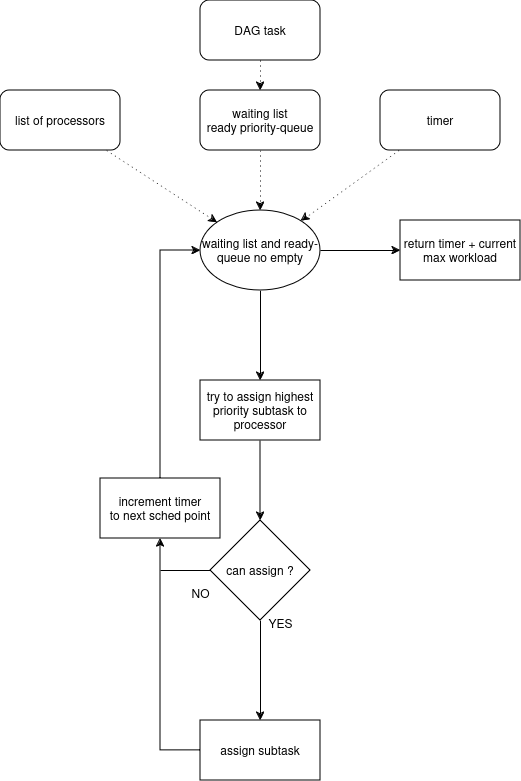
\includegraphics[width=\linewidth]{images/makespan_computation_algorithm_global.png}
    \caption{Top view of the makespan computation algorithm.
    The round squares are inputs and the angular squares are routines or statements.}
    \label{fig:algo_makespan}
\end{figure}

\begin{figure}
    \centering
    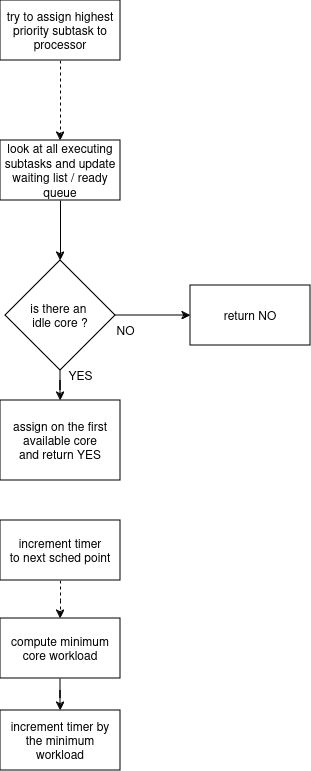
\includegraphics[width=0.8\linewidth]{images/makespan_computation_algorithm_assign.png}
    \caption{Algorithms for assigning the highest priority node (or subtask) to a processor (top)
    and for incrementing the timer to the next scheduling point (bottom).}
    \label{fig:algo_makespan_details}
\end{figure}

The implementation will be done in C++ with bindings to Python to make
the makespan computation faster.

% config for 20,30 nodes : 
%  "dag_config": {
%    "parallelism": 8,
%    "layer_num_min": 5,
%    "layer_num_max": 8,
% config for 10 nodes :
%"dag_config": {
%    "parallelism": 8,
%    "layer_num_min": 3,
%    "layer_num_max": 8,
% config for 40 nodes :
%"dag_config": {
%    "parallelism": 8,
%    "layer_num_min": 7,
%    "layer_num_max": 10,
% config for 50 nodes :
%"dag_config": {
%    "parallelism": 8,
%    "layer_num_min": 10,
%    "layer_num_max": 15,
%config for varying number of parallelism (n=30nodes)
%"dag_config": {
%    "parallelism": [4-6, 7],
%    "layer_num_min": 8, (5 for p = 7)
%    "layer_num_max": 13, (10 for p = 7)